\chapter{fundamentação teórica}
\label{cap:fundamentacao-teorica}

\section{Análise de Sobrevivência em Tempo Discreto com Redes Neurais}

A análise de sobrevivência, também denominada análise de tempo até o evento (\textit{time-to-event analysis}), é um conjunto de técnicas estatísticas destinadas a modelar o tempo decorrido até a ocorrência de um evento de interesse, considerando explicitamente a presença de censura. No contexto deste trabalho, o evento de interesse é o óbito de causa cardíaca, incluindo Morte Súbita Cardíaca ou falência de bomba cardíaca, e a censura corresponde aos pacientes cujo acompanhamento clínico foi encerrado sem a ocorrência do desfecho fatal, seja por alta hospitalar, perda de seguimento ou término do período de estudo.

A censura é um aspecto estrutural dos dados clínicos longitudinais e não pode ser ignorada: excluir pacientes censurados implica viés de seleção, ao passo que tratá-los como se tivessem experimentado o evento introduz viés de informação. Modelos baseados na verossimilhança para dados com censura à direita (\textit{right-censored likelihood}) resolvem esse problema ao incorporar, para cada paciente, a contribuição probabilística adequada ao seu status observado: a probabilidade de ocorrência do evento no tempo observado, para pacientes com evento, e a probabilidade de sobrevivência até o tempo de censura, para pacientes censurados.

A abordagem adotada neste trabalho é a da análise de sobrevivência em tempo discreto com redes neurais, na qual o eixo temporal contínuo é discretizado em $K$ intervalos
\begin{equation}
	[c_0,c_1),\ [c_1,c_2),\ \ldots,\ [c_{K-1},c_K),
\end{equation}
e a rede neural aprende a distribuição do tempo de falha sobre esses intervalos. Conforme proposto por \citeonline{kvamme2019continuous}, os pontos de corte são definidos pelos quantis da distribuição empírica dos tempos de evento observados, em contraste com o esquema equidistante comumente utilizado. Os autores demonstram que tal estratégia é preferível especialmente em conjuntos de dados de menor dimensão, como o presente estudo com 992 pacientes. Esse esquema de discretização é implementado pela classe \texttt{DiscreteTimeTransform}, que ajusta os cortes com base nos quantis dos tempos dos pacientes com evento e garante que o horizonte temporal seja sempre coberto pelo último intervalo.

A rede neural recebe as covariáveis de cada paciente, incluindo sinais de ECG e dados clínicos, e produz um vetor de logits
\begin{equation}
	\bm{\phi} = (\phi_0, \phi_1, \ldots, \phi_{K-1}) \in \mathbb{R}^K,
\end{equation}
a partir do qual as probabilidades de sobrevivência são computadas de acordo com a parametrização adotada. Três funções de perda foram implementadas e avaliadas comparativamente neste estudo, cada uma correspondendo a uma parametrização distinta da distribuição do tempo de falha: \textit{Logistic-Hazard}, \textit{PMF} e \textit{DeepHitSingle}.

\subsection{Logistic-Hazard}

A formulação \textit{Logistic-Hazard}, denominada \textit{Nnet-Survival} por \citeonline{gensheimer2019scalable}, parametriza a função de risco discreta $h_k$, definida como a probabilidade condicional de o evento ocorrer no intervalo $k$, dado que o paciente sobreviveu até o início desse intervalo. Trata-se de um modelo teoricamente fundamentado na verossimilhança de modelos de sobrevivência em tempo discreto, formulados no contexto sociológico por \citeonline{allison1982discrete} e conectados à regressão logística por \citeonline{efron1988logistic}. A aplicação de redes neurais \textit{feedforward} a esse arcabouço foi explorada por \citeonline{biganzoli1998feedforward} por meio de uma abordagem de regressão logística parcial para dados censurados. \citeonline{gensheimer2019scalable} unificam e formalizam essa linha, propondo o treinamento com gradiente estocástico por mini-batches, o que torna o modelo escalável a grandes conjuntos de dados, e demonstram sua competitividade com modelos como \textit{Cox-nnet} e \textit{DeepSurv}.

Para cada bin temporal $k \in \{0,1,\ldots,K-1\}$, o risco discreto é obtido pela aplicação da função sigmoide sobre o logit correspondente:
\begin{equation}
	h_k = \sigma(\phi_k) = \frac{1}{1 + e^{-\phi_k}}.
\end{equation}
A função de sobrevivência discreta é construída como o produto acumulado dos complementos do risco ao longo dos intervalos precedentes:
\begin{equation}
	S(t_k) = \prod_{j=0}^{k} (1-h_j).
\end{equation}

A função de perda é a log-verossimilhança negativa do modelo de sobrevivência em tempo discreto. Para um paciente com evento ($d_i=1$) no intervalo de índice $k_i$, a contribuição à perda é a log-probabilidade conjunta de ter sobrevivido até $k_i-1$ e de ter falhado em $k_i$:
\begin{equation}
	\ell_i = -\log h_{k_i} - \log S(t_{k_i-1}).
\end{equation}
Para um paciente censurado ($d_i=0$) no intervalo $k_i$, a contribuição é a log-probabilidade de sobrevivência até o momento da censura:
\begin{equation}
	\ell_i = -\log S(t_{k_i}).
\end{equation}
A perda total do \textit{batch} é a média das contribuições individuais:
\begin{equation}
	\bar{\mathcal{L}} = \frac{1}{N}\sum_{i=1}^{N}\ell_i.
\end{equation}

Conforme \citeonline{kvamme2019continuous}, que comparam sistematicamente as parametrizações via hazard discreto e via PMF em simulações e dados reais, a parametrização pelo hazard discreto, correspondente ao \textit{Logistic-Hazard}, apresenta desempenho ligeiramente superior à parametrização pela PMF na maioria dos cenários avaliados, embora ambas sejam competitivas. Essa constatação motivou a inclusão do \textit{Logistic-Hazard} como linha de base primária neste trabalho.

\subsection{PMF --- Probability Mass Function}

A formulação PMF, proposta e analisada por \citeonline{kvamme2019continuous}, parametriza diretamente a função de massa de probabilidade $p_k$ sobre os intervalos de tempo discretizados, tratando a distribuição do tempo de falha como um objeto probabilístico explicitamente normalizado. Em vez de estimar funções de risco condicionais para cada bin individualmente, como na formulação \textit{Logistic-Hazard}, o modelo estima a probabilidade de o evento ocorrer especificamente no intervalo $k$, de forma que $\sum_k p_k = 1$.

Para garantir essa propriedade de normalização ao longo de todo o horizonte temporal, incluindo a possibilidade de sobrevivência além do último intervalo observado, \citeonline{kvamme2019continuous} propõem adicionar um logit artificial $\phi_K=0$ ao vetor de saída da rede e aplicar a função \textit{softmax} sobre o vetor aumentado de dimensão $K+1$:
\begin{equation}
	p_k = \frac{e^{\phi_k}}{\displaystyle\sum_{j=0}^{K} e^{\phi_j}},\quad k=0,1,\ldots,K,
\end{equation}
onde $\phi_K=0$ representa o logit do bin artificial correspondente à sobrevivência além do horizonte de observação. A função de sobrevivência é obtida pela soma acumulada reversa da PMF; isto é, a probabilidade de o paciente sobreviver além do bin $k$ é a soma das probabilidades de evento em todos os bins posteriores:
\begin{equation}
	S(t_k) = \sum_{j=k+1}^{K} p_j.
\end{equation}

A função de perda é a log-verossimilhança negativa baseada nessa distribuição conjunta. Para pacientes com evento ($d_i=1$), penaliza-se a log-probabilidade da massa no bin correto; para censurados ($d_i=0$), penaliza-se a log-probabilidade de sobrevivência além do bin de censura:
\begin{equation}
	\ell_i =
	\begin{cases}
		-\log p_{k_i},    & \text{se } d_i=1, \\
		-\log S(t_{k_i}), & \text{se } d_i=0.
	\end{cases}
\end{equation}

A distinção conceitual fundamental entre PMF e \textit{Logistic-Hazard} reside na estrutura das dependências entre os logits: no \textit{Logistic-Hazard}, cada $\phi_k$ define independentemente o risco no bin $k$ por meio da sigmoide, de modo que a função de sobrevivência emerge como um produto; na PMF, todos os $\phi_k$ competem globalmente via \textit{softmax}, de modo que um aumento do logit em um bin necessariamente reduz a probabilidade dos demais. Essa interdependência torna a PMF conceitualmente mais próxima de uma distribuição de probabilidade discreta genuína, mas impõe ao otimizador um espaço de gradientes mais acoplado.

\subsection{DeepHitSingle}

O DeepHit, proposto por \citeonline{lee2018deephit} para a conferência AAAI 2018, representa um avanço qualitativo em relação às formulações anteriores ao incorporar um termo de perda de ordenação (\textit{ranking loss}) à função objetivo, além do termo de verossimilhança. A motivação central é que a maximização da verossimilhança, objetivo compartilhado pelo \textit{Logistic-Hazard} e pelo PMF, otimiza a qualidade das probabilidades absolutas estimadas, mas não garante que o modelo aprenda a ordenar corretamente os pacientes segundo seu risco relativo. Um modelo pode estar bem calibrado em termos de probabilidades e ainda assim cometer erros sistemáticos de ordenação entre pares de pacientes, o que é clinicamente inaceitável em um sistema de estratificação de risco.

Conforme \citeonline{lee2018deephit}, o DeepHit aprende diretamente a distribuição dos tempos de sobrevivência por meio de uma rede neural profunda, sem assumir qualquer forma paramétrica para o processo estocástico subjacente e permitindo que a relação entre as covariáveis e o risco varie ao longo do tempo. Essas propriedades superam as limitações do modelo de Cox proporcional de risco, que impõe a hipótese de proporcionalidade dos hazards e a invariância temporal dos efeitos das covariáveis.

A função de perda total do DeepHit é uma combinação linear de dois termos complementares:
\begin{equation}
	\mathcal{L}_{\text{total}} = \mathcal{L}_1 + \alpha \mathcal{L}_2.
\end{equation}
O primeiro termo, de log-verossimilhança ($\mathcal{L}_1$), é idêntico à formulação PMF descrita anteriormente, com a adição do logit artificial $\phi_K=0$ e aplicação de \textit{softmax}. Esse termo garante que a distribuição de probabilidade estimada seja globalmente coerente com os desfechos observados.

O segundo termo, a perda de ordenação ($\mathcal{L}_2$), penaliza pares de pacientes $(i,j)$ em que o paciente $i$ faleceu antes do paciente $j$ ($t_i<t_j$, $d_i=1$), mas o modelo atribuiu menor risco cumulativo a $i$ do que a $j$ no instante $t_i$. Para cada par válido, a penalidade é proporcional à função exponencial da diferença de risco:
\begin{equation}
	\eta(i,j) = \exp\!\left(-\frac{F(t_i \mid \mathbf{x}_i) - F(t_i \mid \mathbf{x}_j)}{\sigma_{DH}}\right),
\end{equation}
onde
\begin{equation}
	F(t_k \mid \mathbf{x}) = \sum_{j=0}^{k} p_j(\mathbf{x})
\end{equation}
é a função de distribuição acumulada (CDF) do modelo para o paciente com covariáveis $\mathbf{x}$,e $\sigma_{DH}>0$ é um hiperparâmetro de suavização. A lógica da penalidade é a seguinte: quando $F(t_i \mid \mathbf{x}_i) > F(t_i \mid \mathbf{x}_j)$, isto é, quando o modelo atribui corretamente maior risco cumulativo ao paciente que faleceu primeiro, a diferença é positiva, o expoente é negativo e $\eta \to 0$, produzindo penalidade próxima de zero. Quando a ordenação está incorreta, a diferença é negativa ou nula, o expoente tende a zero e $\eta \to 1$, maximizando a penalidade. A perda de ordenação do \textit{batch} é normalizada pela quantidade de pares válidos:
\begin{equation}
	\mathcal{L}_2 =
	\frac{\displaystyle\sum_{i:\,d_i=1}\sum_{j:\,t_i<t_j}\eta(i,j)}
	{\displaystyle\sum_{i:\,d_i=1}\sum_{j:\,t_i<t_j}1 + \varepsilon}.
\end{equation}

O hiperparâmetro $\alpha$ controla o equilíbrio entre calibração probabilística ($\mathcal{L}_1$) e discriminação relativa ($\mathcal{L}_2$). A minimização conjunta dos dois termos promove modelos que são simultaneamente bem calibrados em probabilidade e capazes de distinguir corretamente pacientes de alto e baixo risco, características essenciais para aplicações de prognóstico clínico.

No presente trabalho, o \textit{DeepHitSingle} designa a variante para risco único (\textit{single risk}), em oposição à formulação original com riscos competitivos (\textit{competing risks}). Adicionalmente, para compensar o desbalanceamento da base de dados, em que eventos cardíacos representam aproximadamente $20{,}67\%$ dos pacientes, aplica-se um fator de ponderação \texttt{peso\_evento = 4.0} sobre as contribuições de pacientes com evento no termo $\mathcal{L}_1$, de modo a elevar proporcionalmente o gradiente produzido por esses casos na otimização.

\section{Arquitetura --- ResNet-18 Unidimensional}

\subsection{Aprendizado Profundo Residual}

As redes neurais residuais (\textit{Residual Networks} --- ResNets) foram propostas por \citeonline{he2016deep} como solução ao problema da degradação observado em redes muito profundas: empiricamente, o aumento indiscriminado da profundidade de uma rede produzia piora no desempenho de treinamento, não apenas de generalização, revelando dificuldades de otimização mais fundamentais do que o sobreajuste. A hipótese de \citeonline{he2016deep} é que é mais fácil para a rede aprender um mapeamento residual $\mathcal{F}(\mathbf{x}) = H(\mathbf{x}) - \mathbf{x}$ do que aprender diretamente o mapeamento original $H(\mathbf{x})$, especialmente quando $H(\mathbf{x}) \approx \mathbf{x}$, isto é, quando a transformação ideal é próxima da identidade. Isso é viabilizado pelas conexões de atalho (\textit{skip connections}), que somam a entrada de cada bloco à sua saída transformada:
\begin{equation}
	\mathbf{y} = \mathcal{F}(\mathbf{x},\{W_i\}) + \mathbf{x}.
\end{equation}

Essas conexões criam caminhos de gradiente diretos ao longo de toda a rede durante a retropropagação, mitigando o desvanecimento do gradiente e permitindo o treinamento estável de arquiteturas com dezenas ou centenas de camadas. \citeonline{he2016deep} demonstram que a ResNet-18 e modelos mais profundos superam consistentemente redes sem conexões residuais de mesma ou maior profundidade, tanto em tarefas de classificação de imagens quanto em detecção de objetos.

A adequação da arquitetura ResNet ao domínio do eletrocardiograma foi demonstrada em trabalhos de referência na área. \citeonline{hannun2019cardiologist} empregaram uma rede residual profunda de 34 camadas para classificação de arritmias em ECGs ambulatoriais de derivação única, atingindo desempenho equivalente ou superior ao de cardiologistas em 12 categorias de ritmo. \citeonline{ribeiro2020automatic} desenvolveram uma ResNet de 9 camadas para o diagnóstico automático do ECG de 12 derivações em mais de dois milhões de registros, demonstrando acurácia de nível especialista em seis categorias de alterações clínicas. Esses trabalhos consolidam a ResNet como arquitetura de referência para o processamento de sinais de ECG e fundamentam sua adoção no presente estudo.

\subsection{Adaptação para Sinais Unidimensionais}

A transposição da ResNet-18 para o domínio de sinais temporais consiste na substituição das convoluções bidimensionais, projetadas para imagens com largura e altura, por convoluções unidimensionais, que operam ao longo do único eixo temporal do sinal de ECG. Todas as demais propriedades arquiteturais são preservadas: estrutura dos blocos residuais, dimensionalidade dos canais, normalização em lote e função de ativação ReLU.

O bloco residual básico (\texttt{BasicBlock1D}) é composto por duas convoluções 1D com kernel de tamanho 3 e preenchimento (\textit{padding}) de 1, garantindo que o comprimento temporal do sinal seja preservado dentro do bloco quando não há \textit{stride}. Entre as convoluções, aplica-se normalização em lote (\textit{Batch Normalization}) e ativação ReLU:
\begin{equation}
	\mathbf{y} = \operatorname{ReLU}\!\left(\operatorname{BN}_2\!\left(\operatorname{Conv}_2\!\left(\operatorname{ReLU}\!\left(\operatorname{BN}_1\!\left(\operatorname{Conv}_1(\mathbf{x})\right)\right)\right)\right) + \operatorname{shortcut}(\mathbf{x})\right).
\end{equation}
A conexão de atalho $\operatorname{shortcut}(\mathbf{x})$ é a identidade quando as dimensões de entrada e saída do bloco coincidem. Quando há mudança de \textit{stride} ou de número de canais, caso em que as dimensões são incompatíveis, aplica-se uma projeção linear por convolução $1\times1$ (\textit{downsample}) ao caminho da identidade, conforme especificado por \citeonline{he2016deep}.

A rede completa (\texttt{ResNet1d}) é organizada da seguinte forma: uma camada de entrada com convolução de kernel 7, \textit{stride} 2 e 64 canais de saída, seguida de normalização em lote, ReLU e \textit{max pooling} com kernel 3 e \textit{stride} 2, responsável pela primeira redução da dimensão temporal. Em seguida, quatro grupos de blocos residuais (\texttt{layer1} a \texttt{layer4}) ampliam progressivamente o número de canais para 64, 128, 256 e 512, com redução adicional do comprimento temporal por \textit{stride} 2 nos grupos 2, 3 e 4. O tensor de entrada tem forma $[\text{batch},1,L]$, correspondendo a uma derivação de ECG por janela de sinal de comprimento $L$, e o tensor de saída tem forma $[\text{batch},512,L']$, onde $L'$ é o comprimento temporal após as subamostragens acumuladas.

\subsection{Remoção do Global Average Pooling e Atenção Temporal}

Na implementação canônica da ResNet-18 para classificação de imagens, a saída da última camada convolucional é submetida a \textit{Global Average Pooling} (GAP), que colapsa a dimensão espacial, ou temporal no caso 1D, por média simples, produzindo um vetor de dimensão fixa independente do tamanho da entrada. No presente trabalho, essa camada foi deliberadamente removida, preservando a dimensão temporal na saída do encoder:
\begin{equation}
	\text{saída do encoder}: [\text{batch},512,L'] \quad \text{(3D, dimensão temporal preservada)}.
\end{equation}

A justificativa para essa decisão é de natureza clínica: o GAP pondera igualmente todos os instantes temporais do sinal de ECG, diluindo indistintamente eventos cardíacos breves e clinicamente relevantes, como batimentos ectópicos, pausas sinusais ou alterações transitórias do segmento ST, que podem ser decisivos para a predição de morte súbita cardíaca. Ao preservar a dimensão temporal, é possível aplicar estratégias de agregação seletiva que concentrem a representação final nas regiões do sinal com maior valor prognóstico.

Para essa finalidade, foi implementado um mecanismo de atenção temporal (\textit{TemporalAttention}) como alternativa ao GAP. Dado o tensor de saída da ResNet $\mathbf{H} \in \mathbb{R}^{B\times512\times L'}$, o módulo computa para cada posição temporal $l \in \{1,\ldots,L'\}$ um escore de atenção escalar por meio de uma pequena rede \textit{feedforward} de duas camadas com ativação tangente hiperbólica:
\begin{equation}
	a_l = \mathbf{v}^{\top}\tanh(W_1\mathbf{h}_l + \mathbf{b}_1) \in \mathbb{R}.
\end{equation}
Os escores são normalizados via \textit{softmax} ao longo do eixo temporal, produzindo pesos de atenção $\mathbf{w_l} = \operatorname{softmax}(a_l)$. O vetor de contexto é então obtido por soma ponderada das representações em cada instante:
\begin{equation}
	\mathbf{v_{\text{ctx}}} = \sum_{l=1}^{L'} \mathbf{w_l}\mathbf{h}_l \in \mathbb{R}^{512}.
\end{equation}

O vetor $\mathbf{v_{\text{ctx}}}$ constitui a representação condensada da janela de ECG, com contribuição proporcional de cada instante temporal à sua relevância prognóstica aprendida pelo modelo. Instantes com padrões morfológicos normais recebem pesos baixos; instantes com alterações relevantes recebem pesos elevados. Na versão atual do modelo (\texttt{ModeloSurvivalHibrido}), por razões de regularização e estabilidade durante o desenvolvimento, o módulo de atenção foi temporariamente substituído por média simples ao longo da dimensão temporal (\texttt{features.mean(dim=2)}), equivalente ao GAP, mas a arquitetura de atenção permanece implementada para comparação experimental futura.

\subsection{Modelo Híbrido de Sobrevivência}

O modelo final integra as representações extraídas do sinal de ECG com as variáveis clínicas e demográficas dos pacientes por meio de uma arquitetura de fusão simétrica. Após a extração de características pelo encoder ResNet-18 1D e a agregação temporal, o vetor de 512 dimensões é comprimido por um módulo gargalo (\textit{ECG bottleneck}) composto por duas camadas lineares com ativação ReLU e \textit{Dropout}, produzindo uma representação de 16 dimensões. Paralelamente, as variáveis clínicas são processadas por uma rede \textit{feedforward} de duas camadas (\textit{clinical net}), também produzindo um vetor de 16 dimensões.

A fusão das duas modalidades ocorre por concatenação, resultando em um vetor de 32 dimensões:
\begin{equation}
	\mathbf{f} = [\mathbf{e}_{16}; \mathbf{c}_{16}] \in \mathbb{R}^{32}
\end{equation}
onde $\mathbf{e}_{16}$ é a representação do ECG após o gargalo e $\mathbf{c}_{16}$ é a representação clínica. O vetor $\mathbf{f}$ é então processado pela camada de saída (\textit{head}), composta por camadas lineares com ReLU e \textit{Dropout},
produzindo os logits $\bm{\phi} \in \mathbb{R}^K$ correspondentes aos $K$ bins temporais.

% A escolha por dimensionalidade igual, 16 para cada modalidade, é uma decisão de projeto deliberada: ela garante que nenhuma das duas fontes de informação domine a fusão por ter maior número de parâmetros ou de dimensões representacionais, estabelecendo uma fusão tardia balanceada (\textit{late fusion}) em que ECG e dados clínicos contribuem com pesos equivalentes a priori. Essa simetria é especialmente relevante neste estudo, dado que o objetivo científico inclui comparar o poder preditivo incremental dos sinais de ECG sobre os dados clínicos isoladamente.

% Alguns autores preferem fazer uma ``fundamentação teórica'' no segundo capítulo, outros, preferem fazer uma ``revisão da literatura''. Entretanto, isto é particular de cada trabalho e o autor deve escolher o título mais adequado para o capítulo. Consultar o orientador é importante para determinar o título apropriado.

% Evite começar da seção secundária, ou seja, não passe direto do título do capítulo para o título da seção secundária. Escreva um texto para introduzir as seções subsequentes. Lembre-se de utilizar primeira letra maiúscula quando estiver se referindo a um objeto com numeração específica como capítulo, seção, subseção, figura, tabela, quadro, equação, normalmente, se escreve a primeira letra maiúscula da palavra do objeto seguido do \textit{label}. Por exemplo, a Seção \ref{sec:citacoes} explica como fazer citações bibliográficas. Observe no código fonte deste texto como foi feita a referência cruzada. Isso permite enumerar a seção do modo automático o que facilita caso novas seções sejam criadas.

% \section{Citações bibliográficas}\label{sec:citacoes}

% Esta frase mostra como citar um livro sobre descargas atmosféricas \cite{rakov2003lightning}. Também podem ser citados \textit{sites} como \citeonline{elat2015densidade}. Você precisa escrever o código da referência no arquivo "referencia.bib" dentro da pasta "elementos-pos-textuais". Veja esse, onde estão alguns exemplos que já foram testados.

% Referenciando outro livro \cite{LangtangenLogg2017}. Texto texto texto texto texto texto texto texto texto texto texto texto texto texto texto texto texto texto texto. Texto texto texto texto texto texto texto texto texto texto texto texto texto texto texto texto texto texto texto. Texto texto texto texto texto texto texto texto texto texto texto texto texto texto texto texto texto texto texto. Texto texto texto texto texto texto texto texto texto texto texto texto texto texto texto texto texto texto texto.

% Referenciando outro site \cite{secretaria1999}. Texto texto texto texto texto texto texto texto texto texto texto texto texto texto texto texto texto texto texto. Texto texto texto texto texto texto texto texto texto texto texto texto texto texto texto texto texto texto texto. Texto texto texto texto texto texto texto texto texto texto texto texto texto texto texto texto texto texto texto. Texto texto texto texto texto texto texto texto texto texto texto texto texto texto texto texto texto texto texto. Citando uma norma \cite{NBR10520:2002}.

% Citação de duas referências que concordam entre si \cite{Almeida2018,Gondim2017}. Texto texto texto texto texto texto texto texto texto texto texto texto texto texto texto texto texto texto texto. Texto texto texto texto texto texto texto texto texto texto texto texto texto texto texto texto texto texto texto. Texto texto texto texto texto texto texto texto texto texto texto texto texto texto texto texto texto texto texto. Texto texto texto texto texto texto texto texto texto texto texto texto texto texto texto texto texto texto texto texto texto texto texto texto texto texto. Citando um manual \cite{manuais1989}.

% Outro tipo de citação é a citação literal ou direta com mais de três linhas. Este tipo de citação deve ser destacada com recuo de $4~cm$ da margem esquerda com letra menor (tamanho 10), sem aspas e com espaçamento simples.  Para exemplificar esse tipo de citação, considere a afirmação de \citeonline{feitosa2016}:
% \begin{citacao}
% 	A cultura é o processo através do qual o homem cria o algo onde antes imperava o nada. Esse algo é toda complexidade de criações simbólicas, de sentidos e significados que damos às coisas e ao mundo. Um ``algo'' que não se sustenta se não se entender os processos culturais como mecanismos de mediação entre nós e os fenômenos. Assim, mais do que apenas um elemento da comunicação, a mediação é, por excelência, cultural. As diversas modalidades de mediação são apenas sotaques diferenciados dessa mediação cultural. Assim é a mediação informacional.
% \end{citacao}

% A afirmação do parágrafo anterior também pode ser reproduzida com a citação na final como mostra o exemplo a seguir:
% \begin{citacao}
% 	A cultura é o processo através do qual o homem cria o algo onde antes imperava o nada. Esse algo é toda complexidade de criações simbólicas, de sentidos e significados que damos às coisas e ao mundo. Um “algo” que não se sustenta se não se entender os processos culturais como mecanismos de mediação entre nós e os fenômenos. Assim, mais do que apenas um elemento da comunicação, a mediação é, por excelência, cultural. As diversas modalidades de mediação são apenas sotaques diferenciados dessa mediação cultural. Assim é a mediação informacional. \cite{feitosa2016}.
% \end{citacao}

%Mais exemplos e opções de citações podem ser encontradas em:
%        https://en.wikibooks.org/wiki/LaTeX/Bibliography_Management
%        https://github.com/cfgnunes/latex-cefetmg/blob/master/latex-cefetmg/03-elementos-pos-textuais/apendices.tex            

% \section{Inserindo figuras}\label{sec:figuras}

% A Figura \ref{fig:reitoria} apresenta a fotografia da reitoria da Universidade Federal do Ceará. Observe a estrutura do código para ver como inserir figuras. No título, comece especificando o tipo de figura. Por exemplo, fotografia, desenho, diagrama, fluxograma, gráfico e etc. O espaçamento entre linhas no título é de $1~pt$ (espaçamento simples), apenas a primeira letra da frase é maiúscula. As demais palavras são escritas com letra maiúsculas somente quando são nomes próprios e não há ponto final.

% As margens do título da figura são delimitadas pelo tamanho da figura. Por isso, procure ajustar o tamanho da figura para preencher a largura delimitada pelas margens esquerda e direita da página que possui $16~cm$ de largura. Não esqueça de indicar fonte da figura. O autor deve evitar deixar figuras pequenas menores do que $7~cm$ de largura.

% A posição da figura deve ser o mais próximo logo após ter sido chamada no texto (a figura nunca deve aparecer antes de ter sido anunciada no texto).

% %troque h pelo b ou t para mudar a posição da figura.
% \begin{figure}[h!]
% 	\captionsetup{width=16cm}%Da mesma largura que a figura
% 	\Caption{\label{fig:reitoria} Fotografia da reitoria da Universidade Federal do Ceará}
% 	\UFCfig{}{
% 		
\includegraphics[width=16cm]{figuras/exemplo-1}
% 	}{
% 		\Fonte{\citeonline{UFC2012}.}
% 	}
% \end{figure}

\section{Aprendizado por Representação Contrastiva}
\label{sec:aprendizado-representacao-contrastiva}

O aprendizado auto-supervisionado por contraste (\textit{self-supervised contrastive learning}) é um paradigma de treinamento em que um modelo aprende representações de dados sem rótulos explícitos, maximizando a similaridade entre diferentes visões aumentadas de uma mesma amostra e minimizando-a em relação a amostras distintas. A motivação central é aprender, a partir de grandes volumes de dados não rotulados, representações que capturem estrutura semântica transferível para tarefas supervisionadas \textit{downstream}, especialmente quando os dados rotulados são escassos.

No contexto deste trabalho, esse paradigma é particularmente relevante: a base de dados MUSIC contém 992 pacientes com registros de ECG Holter de 24 horas, mas apenas 205 deles apresentam o evento de interesse (óbito cardíaco), correspondendo a 20,67\% da amostra. O pré-treinamento auto-supervisionado permite utilizar os sinais de ECG de todos os pacientes, independentemente do status de evento, para aprender representações ricas do sinal cardíaco antes do ajuste fino (\textit{fine-tuning}) supervisionado para a tarefa de sobrevivência.

A família de métodos \textit{Momentum Contrast} (MoCo), desenvolvida pelo Facebook AI Research (FAIR) ao longo de três versões progressivas, constitui a base do pré-treinamento do encoder ResNet-18 1D utilizado neste trabalho. Cada versão endereça limitações específicas da anterior, formando uma progressão coerente que culmina na adaptação para \textit{Vision Transformers}. A implementação adotada consolida os avanços das três versões em um arcabouço unificado, aplicado ao domínio de sinais de ECG unidimensionais.

\subsection{MoCo v1: Contraste como Busca em Dicionário Dinâmico}
\label{subsec:moco-v1}

\citeonline{he2020momentum} propõem o \textit{Momentum Contrast} a partir da perspectiva do aprendizado contrastivo como um problema de busca em dicionário (\textit{dictionary look-up}): dada uma amostra de consulta (\textit{query}) $\mathbf{q}$, o objetivo é identificar, em um dicionário de representações, a chave positiva  $\mathbf{k}_{+}$ correspondente à mesma amostra original entre $\mathbf{K_{\text{queue}}}$ chaves negativas $\{\mathbf{k}_{j}^{-}\}_{j=1}^{\mathbf{K_{\text{queue}}}}$.

A principal contribuição do MoCo v1 é a construção de um dicionário dinâmico por meio de dois mecanismos interdependentes: uma fila (\textit{queue}) de representações e um encoder de chave atualizado por momento (\textit{momentum-updated encoder}).

\subsubsection{Fila de Representações}
\label{subsubsec:fila-representacoes}

O dicionário é mantido como uma fila FIFO (\textit{First-In, First-Out}) de representações de mini-batches anteriores \cite{he2020momentum}. A cada iteração de treinamento, as representações produzidas pelo encoder de chave no mini-batch corrente são enfileiradas, e as representações do mini-batch mais antigo são removidas. Seja $B$ o tamanho do mini-batch; após $\lfloor \mathbf{K_{\text{queue}}}/B \rfloor$  iterações, o dicionário contém aproximadamente $\mathbf{K_{\text{queue}}}$ representações negativas disponíveis para a função de perda.

Essa estrutura desacopla o número de amostras negativas do tamanho do mini-batch, permitindo que $\mathbf{K_{\text{queue}}} \gg B$. No presente trabalho, adota-se $\mathbf{K_{\text{queue}}} = 8192$ e $B = 256$, de modo que o dicionário mantém $\mathbf{K_{\text{queue}}}/B = 32$ mini-batches de histórico. Esse valor de $\mathbf{K_{\text{queue}}}$ é deliberadamente menor do que os $\mathbf{K_{\text{queue}}} = 65536$ usados originalmente no ImageNet \cite{he2020momentum}, refletindo a escala do conjunto de ECG (992 pacientes $\times$ 100 janelas/paciente = 99.200 amostras), onde uma fila excessivamente grande introduziria representações muito desatualizadas.

\subsubsection{Encoder de Momento}
\label{subsubsec:encoder-momento}

O encoder de chave $f_k$ não é atualizado por retropropagação direta, mas sim por média móvel exponencial (\textit{Exponential Moving Average}, EMA) dos parâmetros do encoder de consulta $f_q$ \cite{he2020momentum}:
\begin{equation}
	\theta_k \leftarrow m\,\theta_k + (1 - m)\,\theta_q,
	\label{eq:moco-ema}
\end{equation}
onde $m \in [0,1)$ é o coeficiente de momento, adotado como $m = 0{,}999$ neste trabalho. A Equação~\eqref{eq:moco-ema} implica que, a cada iteração, $\theta_k$ se aproxima de $\theta_q$ com passo relativo de apenas $1 - m = 0{,}001$, ou seja, o encoder de chave evolui $1000\times$ mais lentamente do que o encoder de consulta. Essa atualização lenta garante a consistência das representações armazenadas na fila: chaves produzidas em mini-batches anteriores ainda são representações válidas do espaço aprendido, pois $f_k$ não sofreu saltos abruptos que tornariam as chaves antigas incompatíveis com as consultas correntes.

O valor $m = 0{,}999$ é mais conservador do que os valores $m \in \{0{,}99, 0{,}999\}$ explorados em \citeonline{he2020momentum}, sendo preferível em domínios com alta variabilidade intra-amostra como o ECG Holter de 24 horas, onde o mesmo paciente apresenta morfologias distintas ao longo do dia, pois estabiliza o dicionário frente a oscilações rápidas no encoder de consulta.

\subsubsection{Função de Perda InfoNCE}
\label{subsubsec:infonce}

A função de perda utilizada é a InfoNCE (\textit{Noise Contrastive Estimation}) \cite{oord2018cpc}, que formula o problema contrastivo como uma classificação entre $\mathbf{K_{\text{queue}}}+1$ candidatos: identificar a chave positiva $\mathbf{k}_{+}$ entre um conjunto composto por $\mathbf{k}_{+}$ e $\mathbf{K_{\text{queue}}}$ chaves negativas $\{\mathbf{k}_{j}^{-}\}_{j=1}^{\mathbf{K_{\text{queue}}}}$. A similaridade entre representações é medida pelo produto escalar no espaço $\ell_2$-normalizado:
\begin{equation}
	\mathcal{L}_{\mathrm{InfoNCE}} = -\log
	\frac{\exp\left(\mathbf{q}\cdot\mathbf{k}_{+}/\tau\right)}
	{\exp\left(\mathbf{q}\cdot\mathbf{k}_{+}/\tau\right) + \sum_{j=1}^{\mathbf{K_{\text{queue}}}}\exp\left(\mathbf{q}\cdot\mathbf{k}_{j}^{-}/\tau\right)},
	\label{eq:infonce}
\end{equation}
onde $\tau > 0$ é um hiperparâmetro de temperatura que controla a suavidade (\textit{sharpness}) da distribuição sobre os candidatos. Valores baixos de $\tau$ tornam a distribuição mais concentrada, penalizando mais severamente as chaves negativas com alta similaridade à consulta.

A temperatura adotada é $\tau = 0{,}07$, idêntica à reportada por \citeonline{he2020momentum} como ótima para o ImageNet. No contexto de ECG, a temperatura baixa é justificada pela alta discriminabilidade esperada entre padrões morfológicos distintos, como fibrilação atrial e ritmo sinusal, mas exige que as representações estejam bem normalizadas para evitar saturação dos exponenciais, condição garantida pela normalização $\ell_2$ aplicada nas projeções do modelo.

Na implementação, a perda InfoNCE é computada como uma entropia cruzada categórica padrão (\texttt{nn.CrossEntropyLoss}) sobre os logits $\mathbf{l} \in \mathbb{R}^{\mathbf{K_{\text{queue}}}+1}$, onde a classe correta é sempre o índice 0, correspondente à chave positiva. Os logits são construídos como:
\begin{equation}
	\mathbf{l} = \left[\frac{\mathbf{q}\cdot\mathbf{k}_{+}}{\tau};\frac{\mathbf{q}\cdot\mathbf{k}_{1}^{-}}{\tau};\ldots;\frac{\mathbf{q}\cdot\mathbf{k}_{\mathbf{K_{\text{queue}}}}^{-}}{\tau}\right] \in \mathbb{R}^{\mathbf{K_{\text{queue}}}+1},
	\label{eq:moco-logits}
\end{equation}
de modo que minimizar $\mathcal{L}_{\mathrm{InfoNCE}}$ é equivalente a maximizar a probabilidade \textit{softmax} da classe 0, o que corresponde matematicamente à Equação~\eqref{eq:infonce}.

\subsection{MoCo v2: Cabeça de Projeção MLP e Aumentação Aprimorada}
\label{subsec:moco-v2}

O MoCo v2, proposto por \citeonline{chen2020mocov2}, verifica sistematicamente a eficácia de dois aprimoramentos identificados pelo SimCLR \cite{chen2020simclr} e os incorpora ao arcabouço MoCo, demonstrando que ganhos expressivos são possíveis sem aumentar o custo computacional da fila.

\subsubsection{Cabeça de Projeção Não Linear}
\label{subsubsec:projection-head}

A camada de projeção linear ao final do encoder é substituída por uma rede de duas camadas com ativação ReLU:
\begin{equation}
	\mathbf{z} = W_2\,\operatorname{ReLU}(W_1\,\mathbf{h}),
	\label{eq:projection-head}
\end{equation}
onde $\mathbf{h} \in \mathbb{R}^{d}$ é a representação extraída pelo encoder (\textit{backbone}), $W_1 \in \mathbb{R}^{d_h \times d}$ é a matriz de pesos da camada oculta com dimensão $d_h$, e $\mathbf{z} \in \mathbb{R}^{d_z}$ é o vetor de projeção sobre o qual a perda InfoNCE opera. Na implementação do presente trabalho, adota-se $d_z = 256$, valor do hiperparâmetro \texttt{moco\_dim}.

A cabeça de projeção é utilizada exclusivamente durante o pré-treinamento e descartada no \textit{fine-tuning} supervisionado. A representação transferida para o modelo de sobrevivência é $\mathbf{h}$, não $\mathbf{z}$. A motivação é que a perda contrastiva pode demandar invariâncias, por exemplo invariância a aumentações de amplitude, que não são desejáveis na representação final; a cabeça de projeção absorve essas transformações, preservando a riqueza semântica de $\mathbf{h}$.

\subsubsection{Aumentação de Dados Aprimorada}
\label{subsubsec:aumentacao-aprimorada}

Seguindo \citeonline{chen2020mocov2}, a estratégia de aumentação é enriquecida com perturbações adicionais sobre o sinal. No domínio de ECG unidimensional, essas perturbações são implementadas em GPU pelo módulo \texttt{GPU\_ECG\_Augmenter} com probabilidade de aplicação $p = 0{,}80$, o que significa que, em expectativa, 80\% das janelas de sinal recebem pelo menos uma transformação estocástica a cada passagem.

Dada uma janela de sinal $\mathbf{x} \in \mathbb{R}^{C \times L}$, com $C$ canais e $L = 24000$ amostras correspondentes a 24 segundos a 1000 Hz, duas visões aumentadas independentes são geradas:
\begin{equation}
	\mathbf{x}^{(1)} = \mathcal{T}_1(\mathbf{x}), \qquad \mathbf{x}^{(2)} = \mathcal{T}_2(\mathbf{x}),
	\label{eq:moco-views}
\end{equation}
onde $\mathcal{T}_1, \mathcal{T}_2 \overset{\mathrm{i.i.d.}}{\sim} \mathcal{A}$ são realizações independentes da distribuição de aumentação $\mathcal{A}$. As visões $\mathbf{x}^{(1)}$ e $\mathbf{x}^{(2)}$ constituem o par consulta--chave (\texttt{im\_q}, \texttt{im\_k}) da iteração corrente. Crucialmente, as aumentações são aplicadas após a transferência dos dados para a GPU, eliminando o gargalo de CPU que penalizaria o \textit{throughput} com janelas de 24.000 amostras.

\subsection{MoCo v3: Perda Simétrica e Estabilidade de Treinamento}
\label{subsec:moco-v3}

O MoCo v3, apresentado por \citeonline{chen2021mocov3}, não introduz um método fundamentalmente novo, mas endereça o problema central de instabilidade de treinamento que degrada o aprendizado auto-supervisionado com arquiteturas modernas. A contribuição principal, a perda contrastiva simétrica, é incorporada integralmente na implementação deste trabalho.

\subsubsection{Perda Contrastiva Simétrica}
\label{subsubsec:perda-simetrica}

Enquanto o MoCo v1/v2 computa a perda InfoNCE em uma única direção (consulta $\rightarrow$ chave), o MoCo v3 adota uma perda simétrica com dois termos mutuamente invertidos \cite{chen2021mocov3}:
\begin{equation}
	\mathcal{L}_{\mathrm{sym}} = \frac{1}{2}\,\mathcal{L}_{\mathrm{InfoNCE}}\!\left(f_q(\mathbf{x}^{(1)}), f_k(\mathbf{x}^{(2)})\right) + \frac{1}{2}\,\mathcal{L}_{\mathrm{InfoNCE}}\!\left(f_q(\mathbf{x}^{(2)}), f_k(\mathbf{x}^{(1)})\right).
	\label{eq:moco-sym}
\end{equation}
A Equação~\eqref{eq:moco-sym} trata cada visão alternadamente como consulta e como chave, duplicando o número efetivo de pares positivos por amostra sem aumentar o custo de memória. Além do enriquecimento do sinal de aprendizado, a simetria remove o viés direcional implícito na perda assimétrica, o que é relevante no domínio de ECG, onde $\mathcal{T}_1$ e $\mathcal{T}_2$ são equiprováveis e não existe uma visão canonicamente ``mais limpa'' que a outra.

\subsubsection{Instabilidade de Treinamento e Mitigação}
\label{subsubsec:instabilidade-mitigacao}

\citeonline{chen2021mocov3} identificam que a instabilidade se manifesta como oscilações abruptas na curva de perda (\textit{loss dips}), correlacionadas com quedas de desempenho na avaliação \textit{downstream}. No presente trabalho, três mecanismos complementares de mitigação são empregados.

\textbf{Precisão mista automática (AMP).} O treinamento utiliza \texttt{torch.cuda.amp} com \texttt{GradScaler}, que escala dinamicamente o gradiente para evitar \textit{underflow} em \texttt{float16} sem comprometer a acurácia numérica das atualizações em \texttt{float32}. O escalonador mantém um fator de escala $s_t$ que é multiplicado pelos gradientes antes da retropropagação:
\begin{equation}
	\hat{\mathbf{g}}_t = s_t\,\mathbf{g}_t,
	\label{eq:amp-scaling}
\end{equation}
e ajustado adaptativamente: se nenhum gradiente tornar-se \texttt{inf} ou \texttt{NaN} por \texttt{growth\_interval} iterações, $s_t$ é multiplicado por \texttt{growth\_factor}; se ocorrer \textit{overflow}, o passo é descartado e $s_t$ é reduzido.

\textbf{Otimizador SGD com momento.} O otimizador adotado é o Gradiente Descendente Estocástico com momento $\beta = 0{,}9$ e decaimento de peso $\lambda = 5 \times 10^{-4}$:
\begin{align}
	\mathbf{v}_{t+1} & = \beta\,\mathbf{v}_t - \eta_t\left(\nabla_{\theta}\mathcal{L}_t + \lambda\,\theta_t\right),
	\label{eq:sgd-momentum-v}                                                                                       \\
	\theta_{t+1}     & = \theta_t + \mathbf{v}_{t+1},
	\label{eq:sgd-momentum-theta}
\end{align}
onde $\eta_t$ é a taxa de aprendizado na iteração $t$, inicializada em $\eta_0 = 10^{-3}$. O momento $\beta = 0{,}9$ acumula direções de gradiente consistentes ao longo das iterações, suavizando o caminho de otimização e reduzindo a variância estocástica do mini-batch, o que é especialmente benéfico com $B = 256$ amostras em um espaço de representação de dimensão $d_z = 256$.

\textbf{Escalonamento adaptativo da taxa de aprendizado.} O scheduler \texttt{ReduceLROnPlateau} monitora a perda média por época e reduz $\eta_t$ por um fator de $0{,}5$ quando não há melhora por 30 épocas consecutivas, com piso mínimo $\eta_{\min} = 10^{-6}$:
\begin{equation}
	\eta_{t+1} =
	\begin{cases}
		0{,}5\,\eta_t, & \text{se não houver melhora por 30 épocas}, \\
		\eta_t,        & \text{caso contrário}.
	\end{cases}
	\label{eq:reduce-lr}
\end{equation}
Esse mecanismo adapta automaticamente o passo de otimização à paisagem de perda do pré-treinamento contrastivo, que tipicamente apresenta um platô longo seguido de descida suave, padrão esperado em domínios com distribuição de aumentação $\mathcal{A}$ de alta variância.

\subsection{Síntese do Arcabouço Implementado}
\label{subsec:sintese-moco}

A implementação adotada neste trabalho consolida os três avanços da família MoCo em um único arcabouço denominado \texttt{MoCo\_ResNet1D}. O fluxo computacional de uma iteração pode ser descrito em quatro estágios.

\textbf{Estágio 1: aumentação dupla na GPU.} Dada uma janela de ECG $\mathbf{x} \in \mathbb{R}^{C \times 24000}$ do mini-batch corrente, o \texttt{GPU\_ECG\_Augmenter} produz dois sinais perturbados independentes $\mathbf{x}^{(1)}$ e $\mathbf{x}^{(2)}$ conforme a Equação~\eqref{eq:moco-views}.

\textbf{Estágio 2: codificação e projeção.} As visões são processadas pelos encoders de consulta e chave, respectivamente. Para cada visão $v \in \{1,2\}$, o encoder ResNet-18 1D extrai a representação $\mathbf{h}^{(v)} \in \mathbb{R}^{d}$, e a cabeça de projeção MLP produz o vetor normalizado $\mathbf{z}^{(v)} / \|\mathbf{z}^{(v)}\|_2 \in \mathbb{R}^{256}$.

% \textbf{Estágio 3: construção dos logits e perda simétrica.} Para cada direção,
% os logits $\mathbf{l}^{(v)} \in \mathbb{R}^{K+1}$ são construídos conforme a Equação~\eqref{eq:moco-logits} com as $K = 8192$ chaves da fila

\textbf{Estágio 3: construção dos logits e perda simétrica.} Para cada direção,
os logits $\mathbf{l}^{(v)} \in \mathbb{R}^{\mathbf{K_{\text{queue}}}+1}$ são construídos conforme a Equação~\eqref{eq:moco-logits} com as $\mathbf{K_{\text{queue}}} = 8192$ chaves da fila, e a perda simétrica $\mathcal{L}_{\mathrm{sym}}$ é computada conforme a Equação~\eqref{eq:moco-sym}.

\textbf{Estágio 4: atualização dos parâmetros.} O encoder de consulta $f_q$ é atualizado por retropropagação através de $\mathcal{L}_{\mathrm{sym}}$ via SGD, conforme as Equações~\eqref{eq:sgd-momentum-v}--\eqref{eq:sgd-momentum-theta}, com AMP conforme a Equação~\eqref{eq:amp-scaling}. O encoder de chave $f_k$ é atualizado exclusivamente por EMA, conforme a Equação~\eqref{eq:moco-ema}, com $m = 0{,}999$.

A Tabela~\ref{tab:moco-hparams} sumariza os hiperparâmetros adotados e sua justificativa formal.

\begin{table}[ht]
	\centering
	\caption{Hiperparâmetros do pré-treinamento MoCo no domínio ECG.}
	\label{tab:moco-hparams}
	\small
	\begin{tabular}{>{\raggedright\arraybackslash}p{0.12\textwidth} >{\raggedright\arraybackslash}p{0.13\textwidth} >{\raggedright\arraybackslash}p{0.22\textwidth} >{\raggedright\arraybackslash}p{0.38\textwidth}}
		\toprule
		\textbf{Símbolo}            & \textbf{Valor}     & \textbf{Parâmetro}          & \textbf{Justificativa}                                                 \\
		\midrule
		$\mathbf{K_{\text{queue}}}$ & 8.192              & Tamanho da fila             & Aproximadamente 8\% do conjunto total; evita chaves obsoletas.         \\
		$m$                         & 0,999              & Momento do encoder          & Alta estabilidade para ECG com variabilidade intra-dia.                \\
		$\tau$                      & 0,07               & Temperatura InfoNCE         & Distribuição concentrada; consistente com \citeonline{he2020momentum}. \\
		$d_z$                       & 256                & Dimensão da projeção        & Compromisso entre capacidade e generalização.                          \\
		$B$                         & 256                & Tamanho do mini-batch       & $K_{\text{queue}}/B = 32$ mini-batches de histórico na fila.           \\
		$\eta_0$                    & $10^{-3}$          & Taxa de aprendizado         & SGD com momento; escalonado adaptativamente.                           \\
		$\lambda$                   & $5 \times 10^{-4}$ & Decaimento de peso          & Regularização $\ell_2$ padrão para pré-treinamento.                    \\
		$\beta$                     & 0,9                & Momento SGD                 & Suavização do caminho de otimização.                                   \\
		$L$                         & 24.000             & Comprimento da janela       & 24 s a 1.000 Hz; captura ciclos cardíacos completos.                   \\
		$p$                         & 0,80               & Probabilidade de aumentação & 80\% das amostras recebem perturbação por passagem.                    \\
		\bottomrule
	\end{tabular}
\end{table}

\subsection{Relevância do Arcabouço para o Pré-Treinamento em ECG Holter}
\label{subsec:relevancia-moco-ecg}

A adoção do arcabouço MoCo no pré-treinamento do encoder ResNet-18 1D é motivada por dois fatores estruturais do problema.

O primeiro é a escassez de rótulos positivos: com 205 eventos em 992 pacientes (20,67\%), o treinamento supervisionado direto enfrenta risco de sobreajuste e de sub-representação de padrões morfológicos raros. O pré-treinamento contrastivo utiliza os sinais de todos os 992 pacientes, isto é, $992 \times 100 = 99.200$ janelas de 24 s, para construir representações discriminativas sem qualquer supervisão de sobrevivência. O encoder aprende a distinguir padrões de ECG a partir de 99.200 instâncias, enquanto o \textit{fine-tuning} supervisionado posterior dispõe de apenas 992 rótulos de evento.

O segundo é a vantagem da fila de negativos em cenários de baixa prevalência. A fila com $\mathbf{K_{\text{queue}}} = 8192$ representações garante que, a cada iteração, o encoder enfrenta um espectro amplo de morfologias de ECG como amostras negativas. Em um mini-batch de $B = 256$ amostras com 20,67\% de prevalência de evento, o modelo veria em média apenas aproximadamente 53 amostras do grupo de evento por iteração supervisionada; no pré-treinamento contrastivo, todos os 256 sinais do batch contribuem igualmente como âncoras, com $\mathbf{K_{\text{queue}}} = 8192$  negativos adicionais da fila, independentemente de seu rótulo de sobrevivência.

Após o pré-treinamento, os pesos do encoder $f_q$ são transferidos para o modelo híbrido de sobrevivência (\texttt{ModeloSurvivalHibrido}), onde o parâmetro \texttt{freeze\_encoder} governa se $\theta_q$ permanece congelado durante o \textit{fine-tuning}, favorecendo a regularização em regimes de poucos dados, ou é ajustado conjuntamente com o restante do modelo.


\section{Métricas de Avaliação}

A avaliação rigorosa de modelos de sobrevivência exige métricas distintas das empregadas em problemas de classificação ou regressão tradicionais, em razão de duas particularidades estruturais dos dados de tempo até o evento: a presença de censura à direita, que implica informação parcial sobre parte dos pacientes, e a natureza probabilística e temporal da saída do modelo, que é uma função de sobrevivência $\hat{S}(t \mid \mathbf{x})$ definida ao longo de um horizonte contínuo de tempo, e não um escalar único.

Neste trabalho, três métricas complementares são empregadas: o índice de concordância dependente do tempo ($C^{\text{td}}$), proposto por \citeonline{antolini2005}, que avalia a capacidade discriminativa do modelo; o \textit{Integrated Brier Score} (IBS), introduzido por \citeonline{graf1999} e aprimorado por \citeonline{gerds2006}, que avalia conjuntamente calibração e discriminação por meio do erro quadrático médio ponderado; e o \textit{Integrated Negative Binomial Log-Likelihood} (Int.\ NBLL), formalizado por \citeonline{kvamme2019time} com base nos fundamentos do IBS, que avalia a qualidade probabilística da distribuição estimada. Cada uma dessas métricas captura um aspecto distinto e complementar do desempenho preditivo, e seu uso conjunto proporciona uma avaliação abrangente e robusta dos modelos desenvolvidos.

\subsection{Índice de Concordância Dependente do Tempo ($C^{\text{td}}$)}

O índice de concordância original, proposto por Harrell et al.\ (1982), é a extensão da área sob a curva ROC (AUC-ROC) ao contexto de dados censurados: ele mede a proporção de pares de pacientes comparáveis para os quais o modelo ordena corretamente o risco relativo. Contudo, esse índice original baseia-se em escores de risco escalares, tipicamente a função de risco cumulativo em um instante fixo ou o índice de prognóstico linear, o que o torna inadequado para modelos cujos efeitos das covariáveis variam com o tempo, como os modelos de risco não proporcional implementados neste trabalho.

Para superar essa limitação, \citeonline{antolini2005} propõem o índice de concordância dependente do tempo $C^{\text{td}}$, no qual a totalidade da função de sobrevivência estimada $\hat{S}(t \mid \mathbf{x})$ é utilizada como predição de desfecho, em vez de um único escore escalar. A definição de concordância é reformulada de modo a levar em conta o instante específico de cada comparação: um par de pacientes $(i,j)$ com $T_i<T_j$ e $D_i=1$ é considerado concordante se o modelo atribui, no instante $T_i$, uma probabilidade de sobrevivência menor ao paciente $i$ do que ao paciente $j$, isto é, se $\hat{S}(T_i \mid \mathbf{x}_i) < \hat{S}(T_i \mid \mathbf{x}_j)$. Formalmente:
\begin{equation}
	C^{\text{td}} = P\!\left[\hat{S}(T_i \mid \mathbf{x}_i) < \hat{S}(T_i \mid \mathbf{x}_j) \mid T_i<T_j,\ D_i=1\right].
\end{equation}

Essa definição é mais geral do que a do C-Index de Harrell, pois avalia a ordenação dos riscos no instante do evento de cada par, e não em um instante fixo global, sendo adequada para modelos com hazards não proporcionais e com covariáveis de efeito dependente do tempo. Conforme \citeonline{antolini2005}, essa formulação resume a capacidade discriminativa ao longo de todo o horizonte temporal de acompanhamento.

Valores de $C^{\text{td}}=0{,}5$ indicam poder discriminativo equivalente ao acaso, enquanto $C^{\text{td}}=1{,}0$ indica discriminação perfeita. A estimativa amostral é obtida pela proporção de pares concordantes sobre o total de pares comparáveis, com correção para a censura por meio de pesos IPCW (\textit{Inverse Probability of Censoring Weighting}), assegurando consistência da estimativa mesmo quando a censura é informativa em relação às covariáveis.

Na implementação deste trabalho, o $C^{\text{td}}$ é calculado após agregação dos escores de risco por paciente: como cada paciente contribui com múltiplas janelas de sinal de ECG no \textit{dataloader}, os escores de risco individuais de cada janela são agregados por média antes do cálculo da métrica. Essa decisão garante que o índice de concordância reflita o desempenho ao nível do indivíduo clínico, unidade de análise relevante para o prognóstico, e não ao nível da janela de sinal, que seria conceitualmente inadequado para a tarefa.

\subsection{Integrated Brier Score (IBS)}

O Brier Score foi originalmente proposto por Brier (1950) para avaliar a acurácia de previsões probabilísticas em meteorologia e, posteriormente, adaptado ao contexto da análise de sobrevivência. \citeonline{graf1999} introduzem uma versão dependente do tempo do Brier Score para dados de sobrevivência com censura à direita, definindo-o como o erro quadrático médio entre a probabilidade de sobrevivência estimada e o desfecho binário observado em cada instante $t$:
\begin{equation}
	\operatorname{BS}(t) = \frac{1}{N}\sum_{i=1}^{N}\left[\hat{S}(t \mid \mathbf{x}_i) - \mathbf{1}(T_i>t)\right]^2 \hat{w}_i(t),
\end{equation}
onde $\mathbf{1}(T_i>t)$ é o indicador de sobrevivência do paciente $i$ além do instante $t$, e $\hat{w}_i(t)$ são pesos de ponderação por censura inversa (IPCW), estimados pelo inverso da probabilidade de não censura até o instante $t$ segundo o estimador de Kaplan-Meier. Esses pesos garantem que pacientes censurados antes de $t$ sejam excluídos da avaliação de forma não enviesada: para pacientes com $T_i>t$, ainda em risco, $\hat{w}_i(t)=1/\hat{G}(t)$; para pacientes com evento antes de $t$ ($T_i\leq t$, $D_i=1$), $\hat{w}_i(t)=1/\hat{G}(T_i)$; para censurados antes de $t$ ($T_i\leq t$, $D_i=0$), o peso é zero, pois seu desfecho real é desconhecido.

\citeonline{gerds2006} demonstram que o estimador IPCW de \citeonline{graf1999} é consistente sob a hipótese de independência entre os tempos de censura e os tempos de evento dado as covariáveis, e propõem estimadores modificados baseados em modelos de regressão para a distribuição de censura que preservam a consistência mesmo quando essa independência condicional não se verifica exatamente, cenário relevante em estudos clínicos observacionais como o presente.

O Brier Score no instante $t$ mede conjuntamente calibração e discriminação: um modelo perfeitamente calibrado e com discriminação perfeita produz $\operatorname{BS}(t)=0$; um modelo nulo baseado exclusivamente na curva de Kaplan-Meier da população, sem qualquer covariável individual, serve como referência, tipicamente produzindo $\operatorname{BS}(t)\approx0{,}25$ para eventos com prevalência próxima de 50\%.

O \textit{Integrated Brier Score} (IBS) integra numericamente o $\operatorname{BS}(t)$ ao longo de todos os instantes do horizonte de avaliação $[0,t_{\max}]$, fornecendo uma medida escalar global de desempenho:
\begin{equation}
	\operatorname{IBS} = \frac{1}{t_{\max}}\int_{0}^{t_{\max}} \operatorname{BS}(t)\,dt.
\end{equation}
Valores de IBS menores indicam melhor desempenho. O IBS é calculado neste trabalho via a classe \texttt{EvalSurv} da biblioteca \texttt{pycox} \cite{pycox2019}, implementada em \citeonline{kvamme2019time}, que adota a estimativa IPCW de \citeonline{graf1999} com a correção de consistência de \citeonline{gerds2006} como ponderação padrão.

\subsection{Integrated Negative Binomial Log-Likelihood (Int.\ NBLL)}

O \textit{Negative Binomial Log-Likelihood} (NBLL) integrado é uma métrica de avaliação probabilística baseada em regras de pontuação (\textit{scoring rules}) para dados de sobrevivência. \citeonline{kvamme2019time} a formalizam no contexto de modelos de sobrevivência com redes neurais, utilizando os mesmos fundamentos estatísticos do IBS, mas substituindo o erro quadrático, função de perda de Brier, pela log-verossimilhança binomial negativa como medida de discrepância entre a distribuição estimada e o desfecho observado.

Para cada instante $t$, o NBLL é definido como:
\begin{equation}
	\operatorname{NBLL}(t) = -\frac{1}{N}\sum_{i=1}^{N}\left[\mathbf{1}(T_i>t)\log\hat{S}(t \mid \mathbf{x}_i) + \mathbf{1}(T_i\leq t)\log\!\left(1-\hat{S}(t \mid \mathbf{x}_i)\right)\right]\hat{w}_i(t),
\end{equation}
com os mesmos pesos IPCW $\hat{w}_i(t)$ utilizados no Brier Score. A integração ao longo do horizonte temporal produz o Int.\ NBLL:
\begin{equation}
	\text{Int.\ NBLL} = \frac{1}{t_{\max}}\int_{0}^{t_{\max}} \operatorname{NBLL}(t)\,dt.
\end{equation}

A penalidade logarítmica do NBLL é mais severa do que a penalidade quadrática do IBS para previsões extremamente mal calibradas: enquanto o erro quadrático cresce no máximo até 1, por exemplo para previsão de $\hat{S}=1$ quando o evento já ocorreu, a penalidade logarítmica cresce ilimitadamente, com $-\log(0)\to\infty$. Isso torna o Int.\ NBLL particularmente sensível à concentração e ao posicionamento da distribuição estimada: um modelo que distribui elevada probabilidade de sobrevivência a um paciente que veio a óbito recebe penalidade desproporcional, incentivando o modelo a ser bem calibrado especialmente nas regiões temporais de maior risco.

Do ponto de vista da teoria da decisão, tanto o Brier Score quanto o NBLL são regras de pontuação próprias (\textit{proper scoring rules}) \cite{graf1999}, o que garante que sua minimização induz o modelo a fornecer probabilidades que refletem genuinamente suas crenças sobre o desfecho, e não estratégias que minimizam a penalidade por subestimação ou superestimação sistemática. A integração temporal de ambas as métricas ao longo do horizonte de acompanhamento é adotada por \citeonline{kvamme2019time} como protocolo de avaliação padrão nos experimentos comparativos da biblioteca \texttt{pycox}, o que fundamenta sua adoção no presente trabalho.

\subsection{Complementaridade das Métricas e Protocolo de Avaliação}

As três métricas empregadas neste trabalho capturam dimensões distintas e complementares do desempenho preditivo:
\begin{itemize}
	\item O $C^{\text{td}}$ é uma métrica exclusivamente de discriminação: ele avalia se o modelo é capaz de ordenar corretamente os pacientes por nível de risco, independentemente de quão bem calibradas estejam as probabilidades absolutas. Um modelo que sistematicamente superestima ou subestima a sobrevivência, mas mantém a ordenação correta entre os pacientes, pode exibir $C^{\text{td}}$ elevado com IBS e Int.\ NBLL ruins.
	\item O IBS é uma métrica conjunta de calibração e discriminação: penaliza tanto erros de ordenação quanto desvios das probabilidades absolutas em relação aos desfechos observados, sendo, portanto, mais exigente do que o $C^{\text{td}}$ isoladamente.
	\item O Int.\ NBLL é uma métrica de qualidade probabilística: por ser baseado na log-verossimilhança,
	      é mais sensível a erros nas caudas da distribuição, onde o modelo expressa alta confiança, e penaliza de forma mais intensa as previsões muito mal calibradas do que o IBS.
\end{itemize}

Essa complementaridade é essencial para uma avaliação robusta no contexto clínico deste estudo: um modelo de estratificação de risco para morte súbita cardíaca deve ser simultaneamente discriminativo, capaz de separar pacientes de alto e baixo risco; calibrado, para que as probabilidades estimadas possam ser interpretadas clinicamente; e probabilisticamente coerente, para que as distribuições de tempo de evento reflitam adequadamente a incerteza prognóstica. O uso conjunto das três métricas mitiga o risco de selecionar um modelo que seja excelente em uma dimensão às custas das demais.


% A escolha por dimensionalidade igual, 16 para cada modalidade, é uma decisão de projeto deliberada: ela garante que nenhuma das duas fontes de informação domine a fusão por ter maior número de parâmetros ou de dimensões representacionais, estabelecendo uma fusão tardia balanceada (\textit{late fusion}) em que ECG e dados clínicos contribuem com pesos equivalentes a priori. Essa simetria é especialmente relevante neste estudo, dado que o objetivo científico inclui comparar o poder preditivo incremental dos sinais de ECG sobre os dados clínicos isoladamente.

% Texto1 texto texto texto texto texto texto texto texto texto texto texto texto texto texto texto texto texto texto texto texto texto texto texto texto texto texto texto texto texto texto texto texto texto texto texto texto texto texto texto texto texto texto texto texto1.

% Texto2 texto texto texto texto texto texto texto texto texto texto texto texto texto texto texto texto texto texto. Texto texto texto texto texto texto texto texto texto texto texto texto texto texto texto texto texto texto texto2.

% Texto3 texto texto texto texto texto texto texto texto texto texto texto texto texto texto texto texto texto texto. Texto texto texto texto texto texto texto texto texto texto texto texto texto texto texto texto texto texto texto3.

% Texto4 texto texto texto texto texto texto texto texto texto texto texto texto texto texto texto texto texto texto. Texto texto texto texto texto texto texto texto texto texto texto texto texto texto texto texto texto texto texto4.

% A Figura \ref{fig:sondas} Texto texto texto texto texto texto texto texto texto texto texto texto texto texto texto texto texto texto texto. Texto texto texto texto texto texto texto texto texto texto texto texto texto texto texto texto texto texto texto3.

% \begin{figure}[h!]
% 	\centering
% 	\captionsetup{width=14cm}%Da mesma largura que a figura
% 	\Caption{\label{fig:sondas} Gráfico da Atmosfera Superior}
% 	\UFCfig{}{
% 		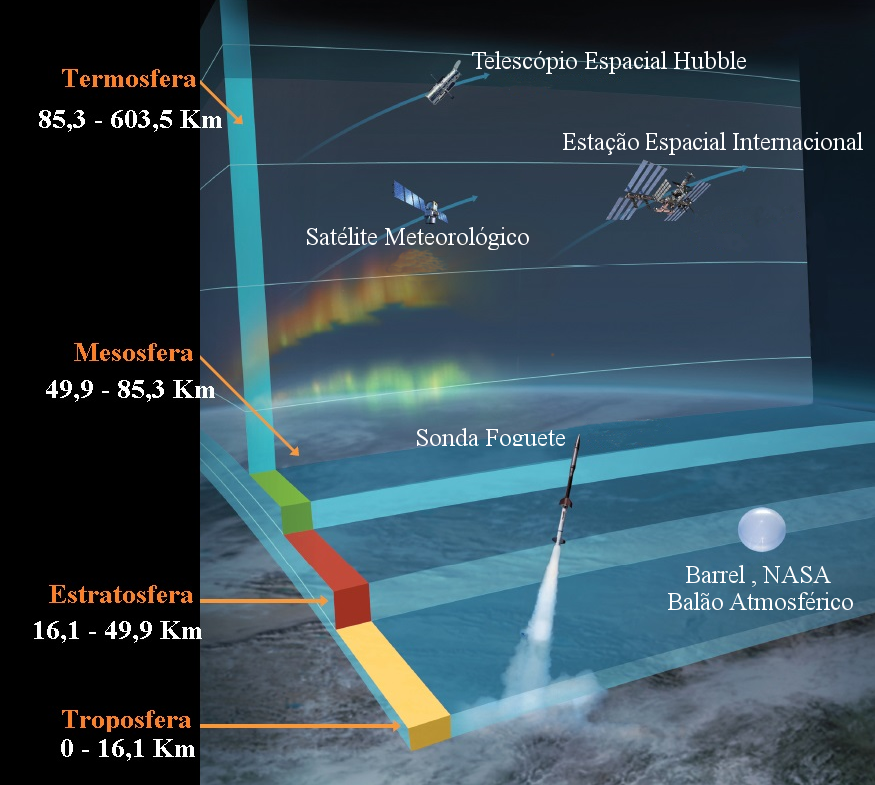
\includegraphics[width=14cm]{figuras/sondas}
% 	}{
% 		\Fonte{adaptado da \citeonline{NASA2016}.}}
% \end{figure}

% Texto5 texto texto texto texto texto texto texto texto texto texto texto texto texto texto texto texto texto texto texto texto texto texto texto texto texto texto texto texto texto texto texto texto texto texto texto texto texto texto texto texto texto texto texto texto5.

% Texto6 texto texto texto texto texto texto texto texto texto texto texto texto texto texto texto texto texto texto texto texto texto texto texto texto texto texto texto texto texto texto texto texto texto texto texto texto texto texto texto texto texto texto texto texto5.

% Texto7 texto texto texto texto texto texto texto texto texto texto texto texto texto texto texto texto texto texto texto texto texto texto texto texto texto texto texto texto texto texto texto texto texto texto texto texto texto texto texto texto texto texto texto texto texto texto texto texto texto texto texto texto texto texto texto texto texto texto texto texto texto texto texto6.

% Evite terminar seções, capítulos e etc com figura. Procure escrever mais.

% \section{Inserindo tabelas}\label{sec:tabelas}

% A Tabela \ref{tab:exemplo-1}... texto texto texto texto texto texto texto texto texto texto texto texto texto texto texto texto texto texto texto. Texto texto texto texto texto texto texto texto texto texto texto texto texto texto texto texto texto texto texto.

% \begin{table}[!h]
% 	\captionsetup{width=7cm}%Deixe da mesma largura que a tabela
% 	\Caption{\label{tab:exemplo-1} Um Exemplo de tabela alinhada que pode ser longa ou curta}%
% 	\IBGEtab{}{%
% 		\begin{tabular}{ccc}
% 			\toprule
% 			Nome           & Nascimento & Documento      \\
% 			\midrule \midrule
% 			Maria da Silva & 11/11/1111 & 111.111.111-11 \\
% 			Maria da Silva & 11/11/1111 & 111.111.111-11 \\
% 			Maria da Silva & 11/11/1111 & 111.111.111-11 \\
% 			\bottomrule
% 		\end{tabular}%
% 	}{%
% 		\Fonte{o autor.}%
% 		\Nota{esta é uma nota, que diz que os dados são baseados na
% 			regressão linear.}%
% 		\Nota[Anotações]{uma anotação adicional, seguida de várias outras.}%
% 	}
% \end{table}

%\begin{table}[h!]	
%	\centering
%	\Caption{\label{tab:exemplo-1} Exemplo de tabela}	
%	\UFCtab{}{
%		\begin{tabular}{cll}
%			\toprule
%			Ranking & Exon Coverage & Splice Site Support \\
%			\midrule \midrule
%			E1 & Complete coverage by a single transcript & Both splice sites\\
%			E2 & Complete coverage by more than a single transcript & Both splice sites\\
%			E3 & Partial coverage & Both splice sites\\
%			E4 & Partial coverage & One splice site\\
%			E5 & Complete or partial coverage & No splice sites\\
%			E6 & No coverage & No splice sites\\
%			\bottomrule
%		\end{tabular}
%	}{
%	\Fonte{elaborado pelo autor.}
%}
%\end{table}

% \subsection{Exemplo de subseção}\label{sec:ex_sec}

% Texto texto texto texto texto texto texto texto texto texto texto texto texto texto texto texto texto texto texto texto texto texto texto texto texto texto texto texto texto texto texto texto texto texto texto texto texto texto texto texto texto texto texto texto texto.

%acrlong{DATASUS},\acrlong{DNV},\acrlong{DO},\acrlong{ESF},\acrlong{IBGE},\acrlong{MFC},\acrlong{MI},\acrlong{MS},\acrlong{NV},\acrlong{ODM},\acrlong{OI},\acrlong{OMS},\acrlong{ONU},\acrlong{PNI},\acrlong{PSF},\acrlong{RIPSA},\acrlong{RN},\acrlong{SIM},\acrlong{SINASC},\acrlong{SUS},\acrlong{TMI},\acrlong{TMMFC}


% \begin{alineascomponto}
% 	\item Integer non lacinia magna. Aenean tempor lorem tellus, non sodales nisl commodo ut
% 	\item Proin mattis placerat risus sit amet laoreet. Praesent sapien arcu, maximus ac fringilla efficitur, vulputate faucibus sem. Donec aliquet velit eros, sit amet elementum dolor pharetra eget
% 	\item Integer eget mattis libero. Praesent ex velit, pulvinar at massa vel, fermentum dictum mauris. Ut feugiat accumsan augue, et ultrices ipsum euismod vitae
% 	\begin{subalineascomponto}
% 		\item Integer non lacinia magna. Aenean tempor lorem tellus, non sodales nisl commodo ut
% 		\item Proin mattis placerat risus sit amet laoreet.
% 	\end{subalineascomponto}
% \end{alineascomponto}

% \subsection{Uso de siglas} \label{sec:siglas}

% Para utilizar siglas, primeiro defina a sigla no arquivo "lista-de-abreviaturas-e-siglas"~ dentro da pasta "1-pre-textuais" com o comando
% \begin{verbatim}
%         \newacronym{ABNT}{ABNT}{Associação Brasileira de Normas Técnicas}
%     \end{verbatim}
% Depois chame a sigla com o comando:
% \begin{verbatim}
%         \gls{ABNT}
%     \end{verbatim}
% Fica assim: \gls{ABNT}. A primeira vez que o comando é usado para uma determinada sigla, aparece o significado por extenso da sigla com a sua abreviação em seguida. A partir da segunda vez que o comando para uma determinada sigla é usado, aparace apenas a sigla. Por exemplo: \gls{ABNT}.

% Veja o código fonte de outros exemplos: Teste de siglas \gls{TEST}, outros exemplos de siglas: \gls{DA}, \gls{MCEG}.
% Repare que sempre as siglas estão sendo definidas primeiramente no arquivo ``lista-de-abreviaturas-e-siglas''.